\documentclass{article}
\usepackage[T1]{fontenc}
\usepackage[utf8]{inputenc}
\usepackage{lmodern}
\usepackage{amsmath}
\usepackage{sansmath}
\AtBeginDocument{\sansmath}
\renewcommand{\familydefault}{\sfdefault}
\usepackage[paperwidth=19cm,paperheight=14cm,margin=0.4cm]{geometry}
\usepackage{graphicx}
\usepackage{tikz}
\usetikzlibrary{positioning,fit,calc,arrows.meta,backgrounds,decorations.pathreplacing}
\pagestyle{empty}
\setlength{\parindent}{0pt}
\graphicspath{{img/}}

\definecolor{ink}{HTML}{0A0A0A}
\definecolor{muted}{HTML}{6A6A69}
\definecolor{line}{HTML}{BDBDBA}
\definecolor{red}{HTML}{E03A3A}
\definecolor{blue}{HTML}{2E6FE0}
\definecolor{yellow}{HTML}{D9A11A}
\definecolor{green}{HTML}{23A06A}
\definecolor{model}{HTML}{8C8C8A}

\tikzset{
  every picture/.style={font=\sffamily\small, line cap=round, line join=round},
  flecha/.style={-{Stealth[length=2.3mm,width=1.7mm]}, line width=0.7pt, draw=ink},
  grupo/.style={draw=#1, dash pattern=on 3pt off 2pt, line width=0.8pt, rounded corners=2pt, inner sep=6pt},
  titulo/.style={font=\sffamily\small\bfseries, text=#1, anchor=south west, inner sep=1pt},
  foto/.style={inner sep=0pt, outer sep=0pt, draw=ink, line width=0.5pt},
  caja/.style={draw=ink, line width=0.5pt, fill=#1, text=white, font=\sffamily\scriptsize\bfseries,
    text width=3.75cm, minimum height=0.46cm, align=center, inner sep=1.5pt},
  nota/.style={font=\sffamily\scriptsize, text=muted, align=center, inner sep=1pt},
  etapa/.style={font=\sffamily\footnotesize\bfseries, text=ink, align=center, inner sep=1pt},
  paso/.style={draw=ink, line width=0.5pt, fill=#1, text=ink, font=\sffamily\scriptsize, align=center,
    inner sep=3pt, minimum height=0.95cm, text width=2.35cm},
  paso/.default=white,
  grupofondo/.style={draw=#1, line width=0.8pt, fill=#1!6, rounded corners=3pt, inner sep=7pt},
  llave/.style={decorate, decoration={brace, mirror, amplitude=5pt, raise=2pt}, line width=0.7pt, draw=#1},
  llavetexto/.style={font=\sffamily\small\bfseries, text=#1, align=center},
}

\begin{document}
\begin{tikzpicture}

\node[foto] (s1) at (0, 0) {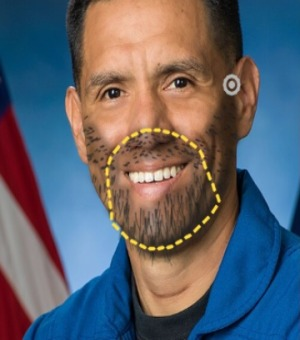
\includegraphics[width=1.8cm]{j_inicio.jpg}};
\node[etapa, above=4pt of s1] {Barba con física};
\node[nota, below=3pt of s1] (n1) {objetivo: candado,\\bigote o collar};

\node[paso, text width=2.2cm, minimum height=1.8cm] (s2) at (2.55, 0) {%
  \textbf{Mano}\\[2pt]MediaPipe Hands;\\corta con el índice\\extendido y el\\medio doblado};

\begin{scope}[shift={(4.55, -0.25)}]
  \draw[blue!16, line width=0.5cm, line cap=round] (0, 0) -- (1.6, 0.5);
  \draw[blue, line width=0.6pt, dash pattern=on 2pt off 1.5pt] (0, 0) -- (1.6, 0.5);
  \fill[ink] (0, 0) circle (0.05) node[below left=-1pt, nota, text=ink] {$p_0$};
  \fill[ink] (1.6, 0.5) circle (0.05) node[above right=-1pt, nota, text=ink] {$p_1$};
  \foreach \x/\y in {0.4/0.15, 0.9/0.25, 1.3/0.45, 0.1/-0.1} { \fill[red] (\x, \y) circle (0.045); }
  \foreach \x/\y in {0.5/0.6, 1.2/-0.3, 0.25/-0.5, 1.75/0.95, -0.2/0.45} { \fill[muted] (\x, \y) circle (0.045); }
  \draw[muted, line width=0.4pt] (1.6, 0.5) -- ++(0.074, -0.238) node[right=0pt, nota] {$r$};
\end{scope}
\node[etapa, anchor=south] at ($(5.35, 0 |- s1.north) + (0, 0.1)$) {Cápsula};
\node[nota] (n3) at (5.35, 0 |- n1) {segmento entre dos\\cuadros, radio $0{,}05\,w$};

\node[foto] (s4) at (8.15, 0) {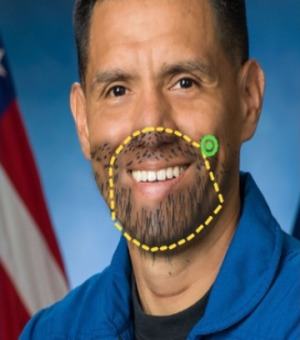
\includegraphics[width=1.8cm]{j_medio.jpg}};
\node[etapa, above=4pt of s4] {Corte};
\node[nota, below=3pt of s4] (n4) {las hebras cortadas\\caen con física};

\node[paso, text width=2.2cm, minimum height=1.8cm] (s5) at (10.7, 0) {%
  \textbf{Puntaje}\\[2pt]$1000 \cdot$ limpieza\\$\cdot$ conservación;\\la IoU daba 0,72\\sin tocar nada};

\node[foto] (s6) at (13.25, 0) {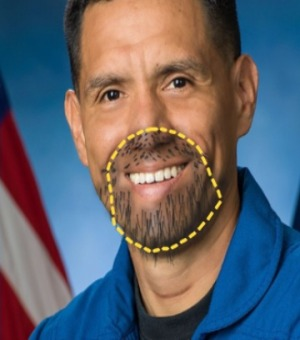
\includegraphics[width=1.8cm]{j_final.jpg}};
\node[etapa, above=4pt of s6] {Final};
\node[nota, below=3pt of s6] (n6) {candado: 827\\puntos};

\draw[flecha] (s1) -- (s2);
\draw[flecha] (s2) -- (4.15, 0);
\draw[flecha] (6.55, 0) -- (s4);
\draw[flecha] (s4) -- (s5);
\draw[flecha] (s5) -- (s6);

\coordinate (base) at ($(n1.south) + (0, -0.06)$);
\draw[llave=muted] (s2.west |- base) -- (s2.east |- base)
  node[midway, below=9pt, llavetexto=muted] {Modelo};
\draw[llave=ink] (4.15, 0 |- base) -- (s5.east |- base)
  node[midway, below=9pt, llavetexto=ink] {Implementado por el equipo};

\end{tikzpicture}
\end{document}
